\documentclass[ ../main.tex]{subfiles}
\providecommand{\mainx}{..}
\begin{document}
\section{Approximate sets}
\label{sec:asets}
Given an objective set $\Set{A}$, any element that is a member of $\Set{A}$ is denoted a \emph{positive} (of $\Set{A})$ and otherwise the element is denoted a \emph{negative}.
Suppose $\hat{\Set{A}}$ is used as an \emph{approximation} of $\Set{A}$.
If the \emph{only} information we have about $\Set{A}$ is given by $\hat{\Set{A}}$, then we may perform membership tests on $\hat{\Set{A}}$ to make \emph{predictions} or \emph{estimations} about $\Set{A}$.

There are two ways a binary prediction can be false.
\begin{enumerate}
    \item A \emph{false positive} occurs if a negative of the objective set is predicted to be a positive. False positives are also known as \emph{type I errors}.
    The complement of false positives are \emph{true negatives}.
    \item A \emph{false negative} occurs if a positive of the objective set is predicted to be a negative. False negatives are also known as \emph{type II errors}.
    The complement of false negatives are \emph{true positives}.
\end{enumerate} 

If we denote the set of false positives by $\PlainSet{FP}$, true positives by $\PlainSet{TP}$, false negatives by $\PlainSet{FN}$, and true negatives by $\PlainSet{TN}$, then the objective set $\Set{A}=\SetUnion[\PlainSet{FN}][\Set{TP}]$ and the approximate set $\hat{\Set{A}}=\SetUnion[\PlainSet{TP}][\PlainSet{FP}]$.
See \cref{fig:ex_approx_set} for an illustration.
\begin{figure}[ht]
\caption{An approximate set $\hat{\Set{A}}$ of an objective set $\Set{A}$}
\label{fig:ex_approx_set}
\centering
\def\svgwidth{\columnwidth/4}
%% Creator: Inkscape inkscape 0.92.1, www.inkscape.org
%% PDF/EPS/PS + LaTeX output extension by Johan Engelen, 2010
%% Accompanies image file 'aset_fp_fn.pdf' (pdf, eps, ps)
%%
%% To include the image in your LaTeX document, write
%%   \input{<filename>.pdf_tex}
%%  instead of
%%   \includegraphics{<filename>.pdf}
%% To scale the image, write
%%   \def\svgwidth{<desired width>}
%%   \input{<filename>.pdf_tex}
%%  instead of
%%   \includegraphics[width=<desired width>]{<filename>.pdf}
%%
%% Images with a different path to the parent latex file can
%% be accessed with the `import' package (which may need to be
%% installed) using
%%   \usepackage{import}
%% in the preamble, and then including the image with
%%   \import{<path to file>}{<filename>.pdf_tex}
%% Alternatively, one can specify
%%   \graphicspath{{<path to file>/}}
%% 
%% For more information, please see info/svg-inkscape on CTAN:
%%   http://tug.ctan.org/tex-archive/info/svg-inkscape
%%
\begingroup%
  \makeatletter%
  \providecommand\color[2][]{%
    \errmessage{(Inkscape) Color is used for the text in Inkscape, but the package 'color.sty' is not loaded}%
    \renewcommand\color[2][]{}%
  }%
  \providecommand\transparent[1]{%
    \errmessage{(Inkscape) Transparency is used (non-zero) for the text in Inkscape, but the package 'transparent.sty' is not loaded}%
    \renewcommand\transparent[1]{}%
  }%
  \providecommand\rotatebox[2]{#2}%
  \ifx\svgwidth\undefined%
    \setlength{\unitlength}{437.78998862bp}%
    \ifx\svgscale\undefined%
      \relax%
    \else%
      \setlength{\unitlength}{\unitlength * \real{\svgscale}}%
    \fi%
  \else%
    \setlength{\unitlength}{\svgwidth}%
  \fi%
  \global\let\svgwidth\undefined%
  \global\let\svgscale\undefined%
  \makeatother%
  \begin{picture}(1,1.05361373)%
    \put(-0.00881474,0.603155){\color[rgb]{0,0,0}\makebox(0,0)[lb]{\smash{}}}%
    \put(-0.01615682,0.61783922){\color[rgb]{0,0,0}\makebox(0,0)[lb]{\smash{}}}%
    \put(0,0){\includegraphics[width=\unitlength,page=1]{aset_fp_fn.pdf}}%
    \put(0.78,0.06){\color[rgb]{0,0,0}\makebox(0,0)[lb]{\smash{$\Set{S} = \SetUnion[\Set{T}[p]][\Set{F}[n]]$}}}%
    \put(0.01737703,1.02584642){\color[rgb]{0,0,0}\makebox(0,0)[lb]{\smash{$\ASet{S} = \SetUnion[\Set{T}[p]][\Set{F}[p]]$}}}%
    \put(0.67844448,0.84067833){\color[rgb]{0,0,0}\makebox(0,0)[lb]{\smash{$\Set{F}[p]$}}}%
    \put(0.84976816,0.43053962){\color[rgb]{0,0,0}\makebox(0,0)[lb]{\smash{$\Set{F}[n]$}}}%
    \put(0.50885122,0.45649776){\color[rgb]{0,0,0}\makebox(0,0)[lb]{\smash{$\Set{T}[p]$}}}%
    \put(0.03987408,0.45476734){\color[rgb]{0,0,0}\makebox(0,0)[lb]{\smash{$\Set{T}[n]$}}}%
    \put(0,0){\includegraphics[width=\unitlength,page=2]{aset_fp_fn.pdf}}%
  \end{picture}%
\endgroup%

\end{figure}

If we only have access to the approximation $\hat{\Set{A}}$, we do not have the ability to partition the universe into the disjoint sets $\PlainSet{FP}$, $\PlainSet{TP}$, $\PlainSet{FN}$, and $\PlainSet{TN}$ as demonstrated in \cref{fig:ex_approx_set}.
However, we can quantify the degree of \emph{uncertainty} about the elements that it predicts to be positive or negative.
The false positive and true negative rates are given by the following.
\begin{definition}
\label{def:fprate}
The \emph{false positive rate} is the proportion of predictions that are \emph{false positives} as given by
\begin{equation}
     \hat{\fprate} = \frac{\Card{\PlainSet{FP}}}{\Card{\PlainSet{FP}} + \Card{\PlainSet{TN}}}
\end{equation}
and the \emph{true negative rate} is given by $\hat{\tnrate} = 1 - \hat{\fprate}$.
\end{definition}
The true positive and false negative rates are given by the following.
\begin{definition}
The \emph{true positive rate} is the proportion of predictions that are \emph{true positives} as given by
\begin{equation}
\hat{\tprate} = \frac{\Card{\PlainSet{TP}}}{\Card{\PlainSet{TP}} + \Card{\PlainSet{FN}}}
\end{equation}
and the \emph{false negative rate} is given by $\hat{\fnrate} = 1 - \hat{\tprate}$.
\end{definition}

The \emph{probabilities} of the four possible predictive outcomes are given by 
\cref{tbl:contingency_table}.
\begin{table}[ht]
\centering
\begin{tabular}{@{} l l l @{}}
    \toprule
    & \textbf{positive} & \textbf{negative}\\
    \midrule
    \textbf{predict positive} & $\hat{\tprate}=1-\hat{\fnrate}$ & 
    $\hat{\fprate}=1-\hat{\tnrate}$\\
    \textbf{predict negative} & $\hat{\fnrate}=1-\hat{\tprate}$ & 
    $\hat{\tnrate}=1-\hat{\fprate}$\\
    \bottomrule
\end{tabular}
\caption{The $2 \times 2$ contingency table of outcomes for approximate sets.}
\label{tbl:contingency_table}        
\end{table}
\end{document}